\chapter{Algorithmen zur Pfadplanung}\index{Algorithmen}\index{Pfadplanung}\index{Algorithmus}
In diesem Kapitel werden zwei der bekanntesten Algorithmen (Dijkstra und Bellman-Ford) zur Pfadplanung beschrieben.

\section{Einleitung}
\label{Was ist Pfadplanung?}
Die Pfadplanung ist ein nichtdeterministisches Problem mit polynomialer Zeit ("NP"), bei dem es darum geht, einen Pfad zu finden, der ein System von seinem Ausgangspunkt zu seinem Ziel verbindet. Der zu wählende Weg (die beste Route) wird durch Beschränkungen und Bedingungen bestimmt\cite{Karur:21}.
\newline
\newline
In der Informatik, insbesondere in der Graphentheorie, ist das Problem des kürzesten Weges bekannt. Der kürzestmögliche Weg von einer Quelle zu einem Ziel hat die geringsten Längenanforderungen.
\newline
\newline
Die Dijkstra- und Bellman-Algorithmen für den kürzesten Weg sind in einer Vielzahl von Bereichen und Anwendungen weit verbreitet. Beispiele für diese Anwendungen sind Routing-Protokolle für Netzwerke, Routenplanung, Verkehrssteuerung, Pfadfindung in sozialen Netzwerken, Computerspiele und Verkehrssysteme\cite{Panda:18}.

\section{Uninformierter Ansatz}\index{uninformiert}
\label{Uninformierter Ansatz}
\subsection{Breitensuche}\index{Breitensuche}
Die Breitensuche gehört zu den uninformierten Suchalgorithmen, diese werden auch „blind“ genannt, weil bei ihrer 
Suche auf keine zusätzlichen Informationen (wie z.B. Wichtungen) zurückgegriffen wird.
Bei der Breitensuche wird zunächst vom Wurzelknoten aus betrachtet alle verbunden Knoten ersten Grades besucht
und dies Ebene für Ebene im Baum\index{Baum} wiederholt bis alle Knoten\index{Knoten} besucht wurden. 
Die Breitensuche findet weitestgehend in der Graphentheorie seine Anwendung.\cite{Russell:10b}
\\
\\
\\
\\
\subsection{Tiefensuche}\index{Tiefensuche}
Die Tiefensuche gehört ebenfalls zu den uninformierten Suchalgorithmen.
Im Gegensatz zu der Breitensuche werden nicht die Ebenen nacheinander abgesucht sondern je Nachfolger angefangen 
beim Wurzelknoten werden bis sie keine weiteren Nachfolger mehr haben besucht. Erst dann wird der nächste Nachbar 
in der ersten Ebene besucht bis keine unbesuchten Knoten mehr vorhanden sind.Die Tiefensuche ist indirekt an vielen 
komplexeren Algorithmen beteiligt. Unter anderem kann die Tiefensuche auch für das Ermitteln von Zusammenhangskomponenten
oder für das Erzeugen eines Irrgartens verwendet werden.
\cite{Russell:10c}


\section{Dijkstra Algorithmus}
\label{Dijkstra Algorithmus}
\subsection{Definition}

Der Dijkstra-Algorithmus (benannt nach seinem Entdecker E.W. Dijkstra) ist ein bekannter Algorithmus auf dem Gebiet der optimalen Pfadwahl und wird verwendet, um den kürzesten Pfad von einem Startpunkt in einem Graphen zu einem Zielpunkt zu finden\cite{Javaid2019}.

\subsection{Funktionsprinzip}

Das Grundkonzept des Algorithmus ist wie folgt:
\newline
\newline
In einem ersten Schritt wird der Startknoten festgelegt und der Abstand zwischen ihm und den anderen Knoten des Graphen berechnet. Gibt es keinen Bogen, der diesen Scheitelpunkt mit dem Startpunkt verbindet, ist der Abstand unendlich; gibt es einen Bogen, der diesen Scheitelpunkt mit dem Startpunkt verbindet, ist der Abstand n; und das niedrigste Gewicht (wenn es mehrere Bögen gibt) ist n.
\newline
\newline
Der zweite Schritt besteht darin, den Punkt mit dem kürzesten Abstand zum Startpunkt zu ermitteln und zu speichern. Die zuvor ermittelte Entfernung wird mit derjenigen verglichen, die über den soeben beiseite gelegten Scheitelpunkt für alle verbleibenden Scheitelpunkte ermittelt wurde, und nur der kleinste der beiden Werte wird beibehalten. Dieser Vorgang wird so lange wiederholt, bis es keine Scheitelpunkte mehr gibt oder bis der Ankunftsscheitelpunkt gewählt ist\cite{Zhou:19}.

\subsection{Vor- und Nachteile}

Der Dijkstra-Algorithmus hat zwei wesentliche Vorteile: Er kann alle optimalen Pfade finden und die Trefferquote dieser optimalen Pfade liegt bei 100 \%. Der zweite Vorteil ist, dass er die verbleibenden unerwünschten Knoten nicht besucht, wenn der beabsichtigte Zielknoten erreicht ist\cite{Zhou:19,Abusalim2020}.
\newline
\newline
Der Hauptnachteil des Algorithmus besteht darin, dass er eine blinde Suche durchführt, was eine erhebliche Menge an Zeit und Ressourcen vergeudet. Ein weiterer Nachteil ist, dass er nicht mit negativen Kanten umgehen kann, was zu azyklischen Graphen führt, und daher nicht immer den kürzesten Weg findet\cite{Mukhlif2020}.

\subsection{Pseudo-Code}

Der Dijkstra-Algorithmus arbeitet mit der Zuweisung einiger vorläufiger Entfernungswerte und versucht, diese schrittweise zu verbessern. Der Pseudocode des Algorithmus ist in der Abbildung \ref{fig:Dijkstra Pseudo-Code}  dargestellt\cite{Huang2012}.
\newline
\newline
Im Folgenden wird die Umsetzung des unten stehenden Pseudocodes erläutert, angelehnt an  \cite{Abusalim2020}.
\newline
Beim Dijkstra-Algorithmus ist die Route unbekannt. Die Knoten werden als temporär (t) oder permanent (p) eingestuft.
\begin{itemize}
	\item  Schritt1: die Entfernung des Quellknotens wird der Wert Null zugewiesen [distance (source) = 0], und die Entfernung der anderen Knoten wird auf unendlich gesetzt [distance(x) = Infinity].
	\item Schritt 2: Suche des Knotens x mit der kürzesten Entfernung d(x). Wenn d(x) unendlich ist oder es keine temporären Knoten gibt, wurde der Knoten x als permanent markiert, was bedeutet, dass sich d(x) und sein übergeordneter Wert nicht ändern werden.
	\item Schritt 3: Für jeden temporären Knoten mit dem Label y, der an x angrenzt, wird der folgende Vergleich durchgeführt:

	
\end{itemize}
\begin{gather*} 
		wenn \ d(x) + w (x, y) < d(y)  \ dann \\
		D(y) = d(x) + w (x, y)
\end{gather*}
\newline
Wenn die Entfernung des gekennzeichneten Knotens y größer ist als die Entfernung des gekennzeichneten Knotens x plus Verbindungsgewicht (x, y), wird die Entfernung des gekennzeichneten Knotens y gemäß der Gleichung aktualisiert.

\begin{figure}[H]
	\centering
	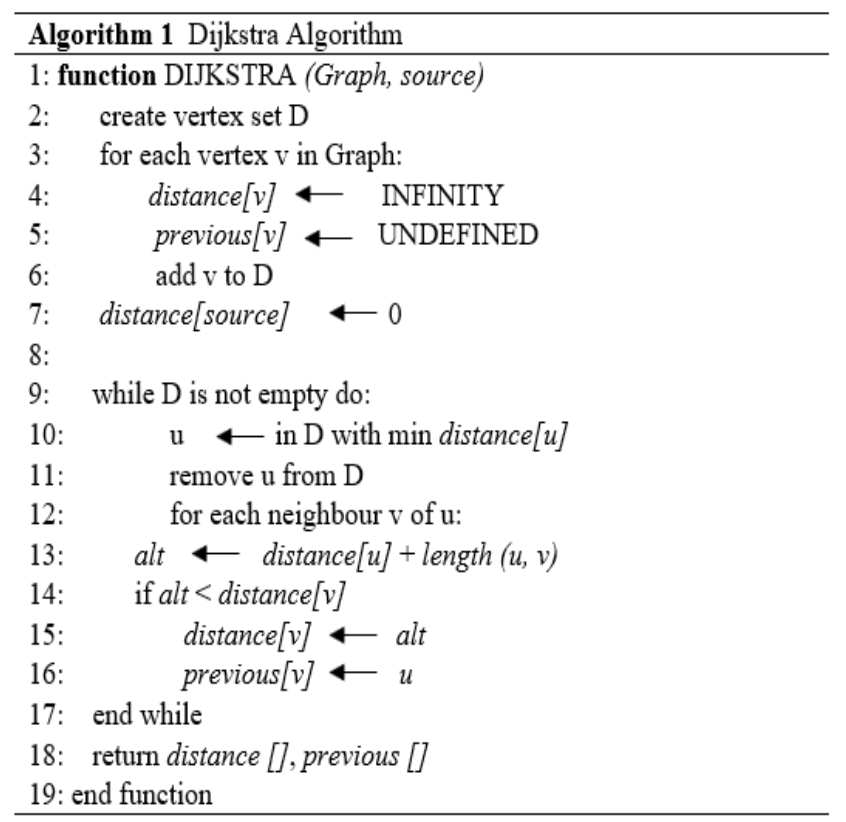
\includegraphics[width=1.0\textwidth]{images/Dijkstra_pseudoCode.PNG}
	\caption{Dijkstra Algorithmus Pseudo-Code, angelehnt an \cite{Abusalim2020}.}
	\label{fig:Dijkstra Pseudo-Code}
\end{figure}




\section{Bellman-Ford Algorithmus}
\label{Bellman-Ford-Algorithmus}
\subsection{Definition}

In 1958 veröffentlichte Richard Bellman den Bellman-Ford-Algorithmus, einen Graphen-Suchalgorithmus zur Ermittlung des kürzesten Pfades.\cite{Abusalim2020,Sulaiman18}.
\subsection{Eigenschaften}
Um kürzeste Wege auf gerichteten Graphen zu finden, nutzt der Bellman-Ford-Algorithmus die Entspannung. Er hat auch einige negative Kanten. Wenn es Zyklen mit negativem Gewicht gibt, wird der Algorithmus sie erkennen (so dass es keine Lösung gibt)\cite{Vaibhavi2014}.
\newline
Die Vorteile dieses Algorithmus sind unter anderem, dass es sich um einen dynamischen Algorithmus handelt, dass er negative gerichtete Kanten (und auch positive) berechnen kann, dass er die Kosten für den Aufbau des Netzes reduzieren kann, indem er den kürzesten Weg von einem Knoten zum anderen findet, und dass er die Anzahl der aufgebauten Router-Pfad reduzieren kann\cite{Abusalim2020}.

\subsection{Pseudo-Code}\index{Bellman-Ford}

Angelehnt an \cite{Abusalim2020} wird der Bellman-Ford-Algorithmus wie folgt ausgeführt:
\newline
\begin{itemize}
	\item   Schritt 1: Zuweisung des Abstandswertes des Quellpunktes s zu null (distance[s] = 0) und des Abstandswertes der anderen Punkte zu INFINITY.
	\item Schritt 2: Wenn n die Anzahl der Knoten ist, wird jede Kante (n - 1) Mal entspannt. Entspannen bedeutet einfach, dass geprüft wird, ob es möglich ist, den Weg zu dem Knoten, auf den die Kante zeigt, zu verkürzen, und wenn dies der Fall ist, wird der Weg zum Knoten durch den entdeckten Weg ersetzt.
	\item Schritt 3: Mit der N-ten Schleife wird geprüft, ob der Graph negative Zyklen aufweist.
\end{itemize}
Der Bellman-Ford-Algorithmus wird wie in der Abbildung \ref{fig:Bellman-Ford Pseudo-code} unten dargestellt ausgeführt.
\begin{figure}[H]
	\centering
	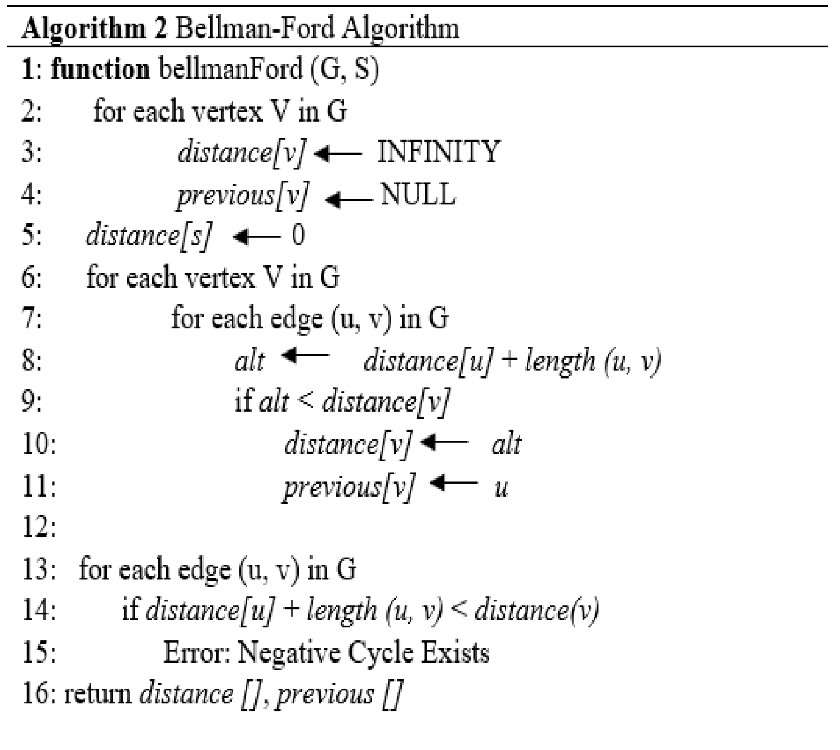
\includegraphics[width=1.0\textwidth]{images/Bellman-Ford-Algorithmus_Pseudo-Code.PNG}
	\caption{Bellman-Ford Pseudo-Code, angelehnt an\cite{Abusalim2020}.}
	\label{fig:Bellman-Ford Pseudo-code}
\end{figure}






